\svnInfo $Id: mmt.tex 19570 2010-04-16 12:48:25Z frabe $
\svnKeyword $HeadURL: https://svn.kwarc.info/repos/kwarc/rabe/Papers/omdoc-spec/MKM_10/mmt.tex $
 
Our representation language {\mmt} was introduced in \cite{rabe:thesis:08}. It arises from three central design goals. Firstly, it should provide an expressive but simple \defemph{module system} as modularity is a necessary requirement for scalability. As usual in language design, the goals of simplicity and expressivity form a difficult trade-off that must be solved by identifying the right primitive module constructs. Secondly, scalability across semantic domains requires \defemph{foundation-independence} in the sense that {\mmt} does not commit to any particular foundation (such as Zermelo-Fraenkel set theory or Church's higher-order logic). Providing a good trade-off between this level of generality and the ability to give a rigorous semantics is a unique feature of {\mmt}. Finally, scalability across implementation domains requires \defemph{standards-compliance}, and while using XML and {\openmath} is essentially orthogonal to the language design, the use of URIs as identifiers is not as it imposes subtle constraints that can be very hard to meet a posteriori.

{\mmt} represents logical knowledge on three levels: On the \defemph{module level}, {\mmt} builds on modular algebraic specification languages for logical knowledge such as OBJ \cite{obj}, ASL \cite{asl}, development graphs \cite{devgraphs}, and CASL \cite{caslmanual}. In particular, {\mmt} uses theories and theory morphism as the primitive modular concepts. Contrary to them, {\mmt} only imposes very lightweight assumptions on the underlying language. This leads to a very simple generic module system that subsumes almost all aspects of the syntax and semantics of specific module systems such as PVS \cite{pvs}, Isabelle \cite{isabelle}, or Coq \cite{coq}.

On the \defemph{symbol level}, {\mmt} is a simple declarative language that uses named symbol declarations where symbols may or may not have a type or a definiens. By experimental evidence, this subsumes virtually all declarative languages. In particular, {\mmt} uses the Curry-Howard correspondence \cite{curry,howard} to represent axioms and theorem as constants, and proofs as terms. Sets of symbol declarations yield theories and correspond to {\openmath} content dictionaries.

On the \defemph{object level}, {\mmt} uses the formal grammar of {\openmath} \cite{openmath} to represent mathematical objects without committing to a specific formal foundation. The semantics of objects is given proof theoretically using judgments for typing and equality between objects. {\mmt} is parametric in these judgments, and the precise choice is relegated to a \defemph{foundation}.
 
\subsection{Module System}\label{sec:mmttnt:modules}

Sophisticated mathematical reasoning usually involves several related but different mathematical contexts, and it is desirable to exploit these relationships by moving theorems between contexts. It is well-known that modular design can reduce space to an extent that is exponential in the depth of the reuse relation between the modules, and this applies in particular to the large theory hierarchies employed in mathematics and computer science.

The first applications of this technique in mathematics are found in the works by Bourbaki (\cite{bourbakisets,bourbakialgebra}), which tried to prove every theorem in the context with the smallest possible set of axioms. {\mmt} follows the ``little theories approach'' proposed in \cite{littletheories}, in which separate contexts are represented by separate \defemph{theories}, and structural relationships between contexts are represented as \defemph{theory morphisms}, which serve as conduits for passing information (e.g., definitions and theorems) between theories (see~\cite{farmerintertheory}). This yields \defemph{theory graphs} where the nodes are theories and the paths are theory morphisms.

\begin{wrapfigure}{r}{7cm}
\begin{center}\vspace*{-4em}\footnotesize
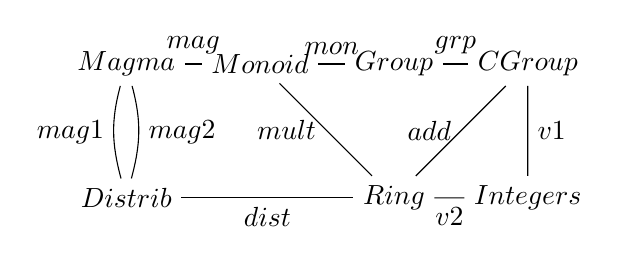
\begin{tikzpicture}[scale=.85]
\node (M)  at (0,0) {$\cn{Magma}$};
\node (Mo) at (2,0) {$\cn{Monoid}$};
\node (G)  at (4,0) {$\cn{Group}$};
\node (GA) at (6,0) {$\cn{CGroup}$};
\node (R)  at (4,-2){$\cn{Ring}$};
\node (D)  at (0,-2){$\cn{Distrib}$};
\node (I)  at (6,-2){$\cn{Integers}$};
\draw[-\arrowtip](M)  --node[above] {$\cn{mag}$} (Mo);
\draw[-\arrowtip](Mo) --node[above] {$\cn{mon}$} (G);
\draw[-\arrowtip](G)  --node[above] {$\cn{grp}$} (GA);
\draw[-\arrowtip](GA) --node[left] {$\cn{add}$} (R);
\draw[-\arrowtip](Mo) --node[left] {$\cn{mult}$} (R);
\draw[-\arrowtip](M) to[out=-105,in=105] node[left] {$\cn{mag1}$} (D);
\draw[-\arrowtip](M) to[out=-75,in=75] node[right] {$\cn{mag2}$}(D);
\draw[-\arrowtip](D)  --node[below] {$\cn{dist}$} (R);
\draw[-\arrowtip](GA)  --node[right] {$\cn{v1}$} (I);
\draw[-\arrowtip](R)  --node[below] {$\cn{v2}$} (I);
\end{tikzpicture}\vspace*{-1em}
\caption{Algebraic Hierarchy}\label{fig:mmttnt:algebra}\vspace*{-2em}
\end{center}
\end{wrapfigure}

\begin{example}[Algebra]\label{ex:mmttnt:algebra}
For example, consider the theory graph in Fig.~\ref{fig:mmttnt:algebra} for a portion of algebra, which was formalized in {\mmt} in \cite{DHK:algebra:09}. It defines the theory of magmas (A magma has a binary operation without axioms.) and extends it successively to monoids, groups, and commutative groups. Then the theory of rings is formed by importing from both $\cn{CGroup}$ (for the additive operation) and $\cn{Monoid}$ (for the multiplicative operation).

A crucial property here is that the imports are named, e.g., $\cn{Monoid}$ imports from $\cn{Magma}$ via an import named $\cn{mag}$. While redundant in some cases, it is essential in $\cn{Ring}$ where we have to distinguish two theory morphisms from $\cn{Monoid}$ to $\cn{Ring}$: The composition $\cnpath{add,grp,mon}$ for the additive monoid and $\cnpath{mult}$ for the multiplicative monoid.

The import names are used to form qualified names for the imported symbols. For example,
if $*$ is the name of the binary operation in $\cn{Magma}$, then
$\cnpath{add,grp,mon,mag,*}$ denotes addition and $\cnpath{mult,mag,*}$ multiplication in $\cn{Ring}$. Of
course, {\mmt} supports the use of abbreviations instead of qualified names, but it is a crucial prerequisite for scalability to make qualified names the default: Without named imports, every time we add a new name in
$\cn{Magma}$ (e.g, for an abbreviation or a theorem), we would have to add corresponding
renamings in $\cn{Ring}$ to avoid name clashes.

Another reason to use named imports is that we can use them to instantiate imports with
theory morphisms. In our example, distributivity is stated separately as a theory that
imports two magmas. Let us assume, the left distributivity axiom is stated as
\[\forall x,y,z.
   x\;\cnpath{mag1,*}\;(y\;\cnpath{mag2,*}\;z)=(x\;\cnpath{mag1,*}\;y)\;\cnpath{mag2,*}\;(x\;\cnpath{mag1,*}\;z)
\]
Then the import $dist$ from $\cn{Distrib}$ to $\cn{Ring}$ will carry the instantiations
$\maps{\cn{mag1}}{\cnpath{mult,mag}}$ and
$\maps{\cn{mag2}}{\cnpath{\cnpath{add,grp,mon,mag}}}$.

In other module systems such as SML, such instantiations are called (asymmetric) sharing declarations.
In terms of theory morphism, their semantics is a commutative diagram, i.e., an equality between
two morphisms such as $\cnpath{dist,mag1}=\cnpath{mult,mag}:\cn{Magma}\arr\cn{Ring}$. This
provides {\mmt} users and systems with a module level invariant for the efficient structuring of
large theory graphs.

Besides imports, which induce theory morphisms into the containing theory, there is a second kind of edge in the theory graph: Views are explicit theory morphisms that represent translations between two
theories. For example, the node on the right side of the graph represents a theory for the
integers, say declaring the constants $0$, $+$, $-$, $1$, and $\cdot$. The fact that the
integers are a commutative group is represented by the view $\cn{v1}$: If we assume that
$\cn{Monoid}$ declares a constant $e$ for the unit element and $\cn{Group}$ a constant
$\cn{inv}$ for the inverse element, then $\cn{v1}$ carries the instantiations
$\maps{\cnpath{grp,mon,mag,*}}{+}$, $\maps{\cnpath{grp,mon,e}}{1}$, and
$\maps{\cnpath{grp,inv}}{-}$. Furthermore, every axiom declared or imported in
$\cn{CGroup}$ is mapped to a proof of the corresponding property of the integers.

The view $\cn{v2}$ extends $\cn{v1}$ with corresponding instantiations for multiplication. {\mmt} permits modular views as well: When defining $\cn{v2}$, we can import all instantiations of $\cn{v1}$ using $\maps{\cn{add}}{\cn{v1}}$. As above, the semantics of such an instantiation is a commutative diagram, namely $\�{\cn{add}}{\cn{v2}}=\cn{v1}$ as intended.
\end{example}

The major advantage of modular design is that every declaration --- abbreviations, theorems, notations etc. --- effects \defemph{induced declarations} in the importing theories. A disadvantage is that declarations may not always be located easily, e.g., the addition in a ring is declared in a theory that is four imports away. {\mmt} finds a compromise here: Through qualified names, all induced declarations are addressable and locatable. The process of removing the modularity by adding all these induced declarations to all theories is called \defemph{flattening}.

\begin{experiment}
The formalization in \cite{DHK:algebra:09} uses the Twelf module system (\cite{RS:twelfmod:09}), which is a special case of {\mmt}. Twelf automatically computes the flattened theory graph. The modular theory graph including all axioms and proofs can be written in 180 lines of Twelf code. The flattened graph is computed in less than half a second and requires more than 1800 lines.

The same case study defines two theories for lattices, one based on orderings and one
based on algebra, and gives mutually inverse views to prove the equivalence of the two
theories. Both definitions are modular: Algebraic lattices arise by importing twice from
the theory of semi-lattices; order-based lattices arise by importing the infimum operation
twice, once for the ordering and once for its dual. Consequently, the views can be given
modularly as well, which is particularly important because views must map axioms to
expensive-to-find proofs. These additional declarations take 310 lines of Twelf in modular
and 3500 lines in flattened form.  

These numbers already show the value of modularity in representation already in very small
formalizations. If this is lacking, later steps will face severe scalability problems from
blow-up in representation. Here, the named imports of {\mmt} were the crucial innovation to
strengthen modularity.
\end{experiment}

\subsection{Foundation-Independence}

Mathematical knowledge is described using very different foundations, and the most common foundations can be grouped into set theory and type theory. Within each group there are numerous variants, e.g., Zermelo-Fraenkel or G\"odel-Bernays set theory, or set theories with or without the axiom of choice. Therefore, a single representation language can only be adequate if it is foundation-independent.

{\openmath} and {\omdoc} achieve this by concentrating on structural issues and leaving lexical ones to an external definition mechanism like content dictionaries or theories. In particular, this allows us to operate without choosing a particular foundational logical system, as we can just supply content dictionaries for the symbols in the particular logic. Thus, logics and in the same way foundations become theories, and we speak of the {\defemph{logics-as-theories}} approach.

But conceptually, it is helpful to distinguish levels here. To state a property in the theory $\cn{CGroup}$ like commutativity of the operation $\circ:=\cnpath{grp,mon,mag,*}$ as $\forall a,b.a\circ b=b\circ a$, we use symbols $\forall$ and $=$ from first-order logic together with $\circ$ from $\cn{CGroup}$. Even though it is structurally possible to build algebraic theories by simply importing first-order logic, this would fail to describe the meta-relationship between the theories. But this relation is crucial, e.g., when interpreting $\cn{CGroup}$ in the integers, the symbols of the meta-language are not interpreted because a fixed interpretation is given in the context.

To understand this example better, we use the $M/T$ notation for meta-languages. $M/T$ refers to working in the object language $T$, which is defined within the meta-language $M$. For example, most of mathematics is carried out in $FOL/ZF$, i.e., first-order logic is the meta-language, in which set theory is defined. $FOL$ itself might be defined in a logical framework such as $LF$, and within $ZF$, we can define the language of natural numbers, which yields $LF/FOL/ZF/Nat$. For algebra, we obtain, e.g., $FOL/\cn{Magma}$. {\mmt} makes this meta-relation explicit: Every theory $T$ may point to another theory $M$ as its meta-theory. We can write this as $MMT/(M/T)$.

\begin{wrapfigure}{r}{6cm}\vspace*{-2em}
\fbox{
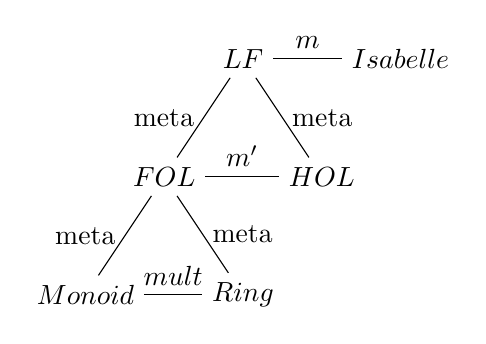
\begin{tikzpicture}
\node (A) at (0,3)  {$\cn{LF}$};
\node (A') at (2,3)  {$\cn{Isabelle}$};
\node (C) at (-1,1.5)   {$\cn{FOL}$};
\node (C') at (1,1.5) {$\cn{HOL}$};
\node (E) at (-2,0) {$\cn{Monoid}$};
\node (E') at (0,0)  {$\cn{Ring}$};
\draw(A) --node[left] {meta} (C);
\draw(A) --node[right] {meta} (C');
\draw(C) --node[left] {meta} (E);
\draw(C) --node[right] {meta} (E');
\draw[-\arrowtip](A) --node[above] {$m$} (A');
\draw[-\arrowtip](C) --node[above] {$m'$} (C');
\draw[-\arrowtip](E) --node[above] {$\cn{mult}$} (E');
\end{tikzpicture}
}\vspace*{-.5em}
\caption{Meta-Theories}\label{fig:mmt:intro:metatheory}\vspace*{-1em}
\end{wrapfigure}

In Fig.~\ref{fig:mmt:intro:metatheory}, the algebra example is extended by adding meta-theories. The theory $\cn{FOL}$ for first-order logic is the meta-theory for all algebraic theories, and the theory $\cn{LF}$ for the logical framework LF is the meta-theory of $\cn{FOL}$ and of the theory $\cn{HOL}$ for higher-order logic.

Now the crucial advantage of the logics-as-theories approach is that on all three levels the same module system can be used: For example, the views $m$ and $m'$ indicate possible translations on the levels of logical frameworks and logics, respectively. Similarly, logics and foundations can be built modularly. Thus, we can use imports to represent inheritance at the level of logical foundations and views to represent formal translations between them. Just like in the little theories approach, we can prove meta-logical results in the simplest foundation that is expressive enough and then use views to move results between foundations.

\begin{example}[Little Logics and Little Foundations]\label{ex:mmttnt:foundations}
In \cite{HR:folsound:09}, we formalize the syntax, proof theory, and model theory and prove the soundness of first-order logic in {\mmt}. Using the module system, we can treat all connectives and quantifiers separately. Thus, we can reuse these fragments to define other logics, and in \cite{project:latin} we do that, e.g., for sorted first-order logic and modal logic. 

For the definition of the model theory, we need to formalize set theory in {\mmt}, which is a significant investment, and even then doing proofs in set theory --- as needed for the soundness proof --- is tedious. Therefore, in \cite{HR:folsound:10}, we develop the set theoretical foundation itself modularly. We define a typed higher-order logic $\cn{HOL}$ first, which is expressive enough for many applications such as the above soundness proof. Then a view from $\cn{HOL}$ to $\cn{ZF}$ proves that $\cn{ZF}$ is a refinement of $\cn{HOL}$ and completes the proof of the soundness of FOL relative to models defined in $\cn{ZF}$.
\end{example}

\begin{experiment}
Ex.~\ref{ex:mmttnt:foundations} already showed that it is feasible to represent foundations and relations between foundations in {\mmt}. Being able to this is a qualitative aspect of cross-domain scalability. In another case study, we represented $LF/Isabelle$ and $LF/Isabelle/HOL$ (\cite{isabelle,isabellehol}) as well as a translation from them into $LF/FOL/ZFC$ (see \cite{project:latin}).
\end{experiment}

To our knowledge, {\mmt} is the only declarative formalism in which comparable foundation or logic translations have been conducted. In Hets (\cite{hets}) a number of logic translations are implemented in Haskell. Twelf and Delphin provide logic and functional programming languages, respectively, on top of LF (\cite{twelf,delphin}), which have been used to formalize the HOL-Nuprl translation (\cite{hol_nuprl}).

\subsection{Symbol Identifiers ``in the Large''}

In mathematical languages, we need to be able to refer to (i.e., identify) content objects in order to state the semantic relations. It was a somewhat surprising realization in the design of {\mmt} that to understand the symbol identifiers is almost as difficult as to understand the whole module system. Theories are containers for symbol declarations, and relations between theories define the available symbols in any given theory. Since every available symbol should have a canonical identifier, the syntax of identifiers is inherently connected to the possible relations between theories.

In principle, there are two ways to identify content object: \defemph{by location} (relative to a particular document or file) and \defemph{by context} (relative to a mathematical theory). The first one essentially makes use of the organizational structure of files and file systems, and the second makes use of mathematical structuring principles supplied by the representation format.

As a general rule, it is preferable to use identification by context as the distribution of
knowledge over file systems is usually a secondary consideration. Then the mapping between theory identifiers and physical theory locations can be deferred to an extralinguistic catalog. Resource identification by context should still be compatible with the URI-based approach that mediates most resource transport over the internet. This is common practice in scalable programming languages such as Java where package identifiers are URIs and classes are located using the \texttt{classpath}.

For logical and mathematical knowledge, the {\openmath} 2 standard (\cite{openmath}) and the current {\omdoc} version 1.2 define URIs for symbols. A symbol is identified by the symbol name and content dictionary, which in turn is identified by the CD name and the CD base, i.e., the URI where the CD is located. From these constituents, symbol URIs are formed using URI fragments (the part after the \# delimiter). However, {\openmath} imposes a one-CD-one-file restriction, which is too restrictive in general. While {\omdoc}1.2 permits multiple theories per file, it requires file-unique identifiers for all symbols. In both cases, the use of URI fragments, which are resolved only on the client, forces clients to retrieve the complete file even if only a single symbol is needed.

Furthermore, many module systems have features that impede or complicate the formation of canonical symbol URIs. Such features include unnamed imports, unnamed axioms, overloading, opening of modules, or shadowing of symbol names. Typically, this leads to a non-trivial correspondence between user-visible and application-internal identifiers. But this impedes or complicates cross-application scalability where all applications (ranging from, e.g., a Javascript GUI to a database backend) must understand the same identifiers.
  
{\mmt} avoids the above pitfalls and introduces a simple yet expressive web-scalable syntax for symbol identifiers. An {\mmt}-URI is of the form $doc?mod?sym$ where
\vspace{-.5em}
\begin{itemize}
\item $doc$ is a URI without query or fragment, e.g.,
  \url{http://cds.omdoc.org/math/algebra/algegra1.omdoc} which
  identifies (but not necessarily locates) an {\mmt} document,
\item $mod$ is a $/$-separated sequence of local names that gives the path to a nested
  theory in the above document, e.g., $\cn{Ring}$,
\item $sym$ is a $/$-separated sequence $imp_1/\ldots/imp_n/con$ of local names such that
  $imp_i$ is an import and $con$ a symbol name, e.g., $\cnpath{mult,mon,*}$,
\item a local name is of the form $pchar^+$ where $pchar$ is defined as in RFC
  3986~\cite{uri}, which --- possibly via \%-encoding --- permits almost all Unicode
  characters.
\end{itemize}

In our running example, the canonical URI of multiplication in a ring is
\url{http://cds.omdoc.org/math/algebra/algegra1.omdoc?Ring?mult/mon/*}.\\  Note that the use
of two \url{?} characters in a URI is unusual outside of {\mmt}, but legal w.r.t. RFC 3986.  Of
course, {\mmt} also defines relative URIs that are resolved against the URI of the
containing declaration. The most important case is when $doc$ is empty. Then the
resolution proceeds as in RFC 3986, e.g., $?mod'?sym'$ resolves to $doc?mod'?sym'$
relative to $doc?mod?sym$ (Note that this differs from RFC 2396.). {\mmt} defines some
additional cases that are needed in mathematical practice and go beyond the expressivity
of relative URIs: Relative to $doc?mod?sym$, the resolution of $??sym'$ and $?/mod'?sym'$
yields $doc?mod?sym'$ and $doc?mod/mod'?sym'$, respectively.

\begin{experiment}
URIs are the main data structure needed for cross-application scalability, and our experience shows that they must be implemented by almost every peripheral system, even those that do not implement {\mmt} itself. Already at this point, we had to implement them in SML (\cite{RS:twelfmod:09}), Javascript (\cite{GLR:jobad:09}), XQuery (\cite{ZKR:tntbase:10}), Haskell (for Hets, \cite{hets}), and Bean Shell (for a jEdit plugin) --- in addition to the Scala-based reference API (Sect.~\ref{sec:mmttnt:flomdoc}).

This was only possible because {\mmt}-URIs constitute a well-balanced trade-off between mathematical rigor, feasibility, and URI-compatibility: In particular, due to the use of the two separators $/$ and $?$ (rather than only one), they can be parsed locally, i.e., without access to or understanding of the surrounding {\mmt} document. And they can be dereferenced using standard URI libraries and URI-URL translations. At the same time, they provide canonical names for all symbols that are in scope, including those that are only available through imports.
\end{experiment}


